\documentclass{beamer}
\usepackage[utf8]{inputenc}
\usepackage[spanish]{babel}
\usetheme{metropolis}           % Use metropolis theme
\graphicspath{{images/}}

\usepackage{multicol}
\usepackage{listings}
\usepackage[default]{sourcesanspro}

\usepackage[scale=2]{ccicons}

\usepackage[
    type={CC},
    modifier={by-nc-sa},
    version={4.0},
]{doclicense}



\hypersetup{
    colorlinks=true,
    linkcolor=black,
    filecolor=magenta,
    urlcolor=cyan,
}

\title{Aprendizaje automático de un sistema interpretable de ayuda a la decisión para la estimación de la edad a partir de los huesos del pubis.}

\date{\today}
\author{\small Autor: Antonio David Villegas Yeguas \\ Directores: Óscar Cordón García y Sergio Damas Arroyo}
\institute[UGR]{Universidad de Granada\\
\medskip
\textit{advy99@correo.ugr.es}\\
\medskip
\url{https://github.com/advy99/TFG}
\doclicenseThis
}
\setbeamertemplate{caption}{\raggedright\insertcaption\par}

\begin{document}

 \maketitle

\begin{frame}{Índice}
\tableofcontents
\end{frame}




\section{Introducción y estado del arte del problema}
\begin{frame}{Estimación de la edad a partir de los huesos del pubis}

	\begin{columns}[T]
		\begin{column}{.4\textwidth}
			Problema de gran interés, pero complejo:
			\begin{itemize}
				\item No existe un método concreto.
				\item Trabajo subjetivo por parte de forenses.
				\item Falta de muestras para edades tempranas.
				\item Primera propuesta en 1920 por T. W. Todd \cite{todd}, clasificación en diez fases utilizando nueve características.
			\end{itemize}

		\end{column}

		\begin{column}{.7\textwidth}
			\begin{table}[H]
				\centering
				\resizebox{1\textwidth}{!}{%
					\begin{tabular}{|c|c|c|}
					\hline
					Crestas y surcos: Muy definidos & Superficie porosa irregular: Sí & Borde superior: Definido  \\ \hline
					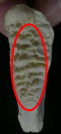
\includegraphics[scale = 0.75]{huesos/crestas_surcos_muy_definidos.png}  &   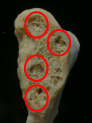
\includegraphics[scale = 0.75]{huesos/superficie_porosa_si.png} &  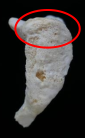
\includegraphics[scale = 0.75]{huesos/borde_superior_definido.png}  \\ \hline
					Nódulo óseo: Presente & Borde inferior: No definido & Borde dorsal: Definido \\ \hline
					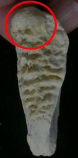
\includegraphics[scale = 0.75]{huesos/nodulo_oseo_presente.png} & 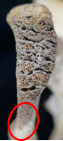
\includegraphics[scale = 0.75]{huesos/borde_inferior_no_definido.png} &  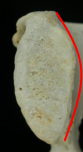
\includegraphics[scale = 0.75]{huesos/borde_dorsal_definido.png} \\ \hline
					Plataforma dorsal: Presente & Bisel ventral: En proceso de formación & Borde ventral: Muchas excrecencias \\ \hline
					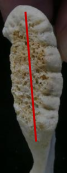
\includegraphics[scale = 0.75]{huesos/plataforma_dorsal_presente.png} & 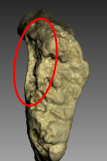
\includegraphics[scale = 0.75]{huesos/bisel_ventral_en_proceso_formacion.png} &   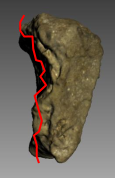
\includegraphics[scale = 0.75]{huesos/borde_ventral_muchas_excrecencias.png} \\ \hline
					\end{tabular}%
				}
				\caption{Algunos ejemplos de las características consideradas por Todd\cite{todd}.}\label{table:caracteristicas_todd}
			\end{table}
		\end{column}

	\end{columns}


\end{frame}

\begin{frame}[allowframebreaks]{Estado del arte}

\begin{itemize}
\item 1953 a 1973: Gilbert y McKern \cite{propuestaGilbert}. Cambio de enfoque a regresión, resultado expresado en un único valor y reducción de características.

\item 1990: J. M. Suchey y S. Brooks. Reducción del número de fases.

\item 2015: D. E. Slice y Algee-Hewitt. Escaneo de huesos utilizando Visión por Computador, clasificación con regresión lineal utilizando la propuesta de Suchey y Brooks. 41 muestras con una RECM de $17,15$ años.

\item 2015: D. Stoyanova, D. E. Slice y Algee-Hewitt. Modificación de las características utilizadas en su trabajo anterior. 57 muestras con una RECM de $19$ años.

\item 2018: A. Kotěrová, D. Navega, M. Štepanovský, Z. Buk, J. Brůžek y E. Cunha. Distintos modelos de aprendizaje, entre ellos regresión lineal, árboles de decisión y redes neuronales. 941 muestras, RECM de $12.1$ años y EAM de $9.7$ años.

\item 2021: J. C. Gámez-Granados, J. Irurita, R. Pérez, A. González, S. Damas, I. Alemán y O. Cordón (sometido a revista). Enfoque de Todd como un problema de clasificación ordinal, aprendizaje basado en reglas de forma iterativa. 892 muestras, RECM de $12,34$ años y 34 reglas fácilmente interpretables.

\end{itemize}

\end{frame}


\section{Objetivos}
\begin{frame}{Objetivos}
Nuestros objetivos serán:

\begin{enumerate}
	\item Obtener resultados sencillos, obtenidos a partir de modelos fácilmente interpretables.
	\item Tratar la alta dimensionalidad del problema.
	\item Resolver el problema del número de muestras del conjunto de datos.
\end{enumerate}

\end{frame}


\section{Inteligencia Artificial Explicable}
\begin{frame}{Inteligencia Artificial Explicable}

	Producir modelos fácilmente interpretables manteniendo buenos resultados y permitir que sean transparentes de cara a entender su funcionamiento.

	\begin{figure}[H]
		\centering
		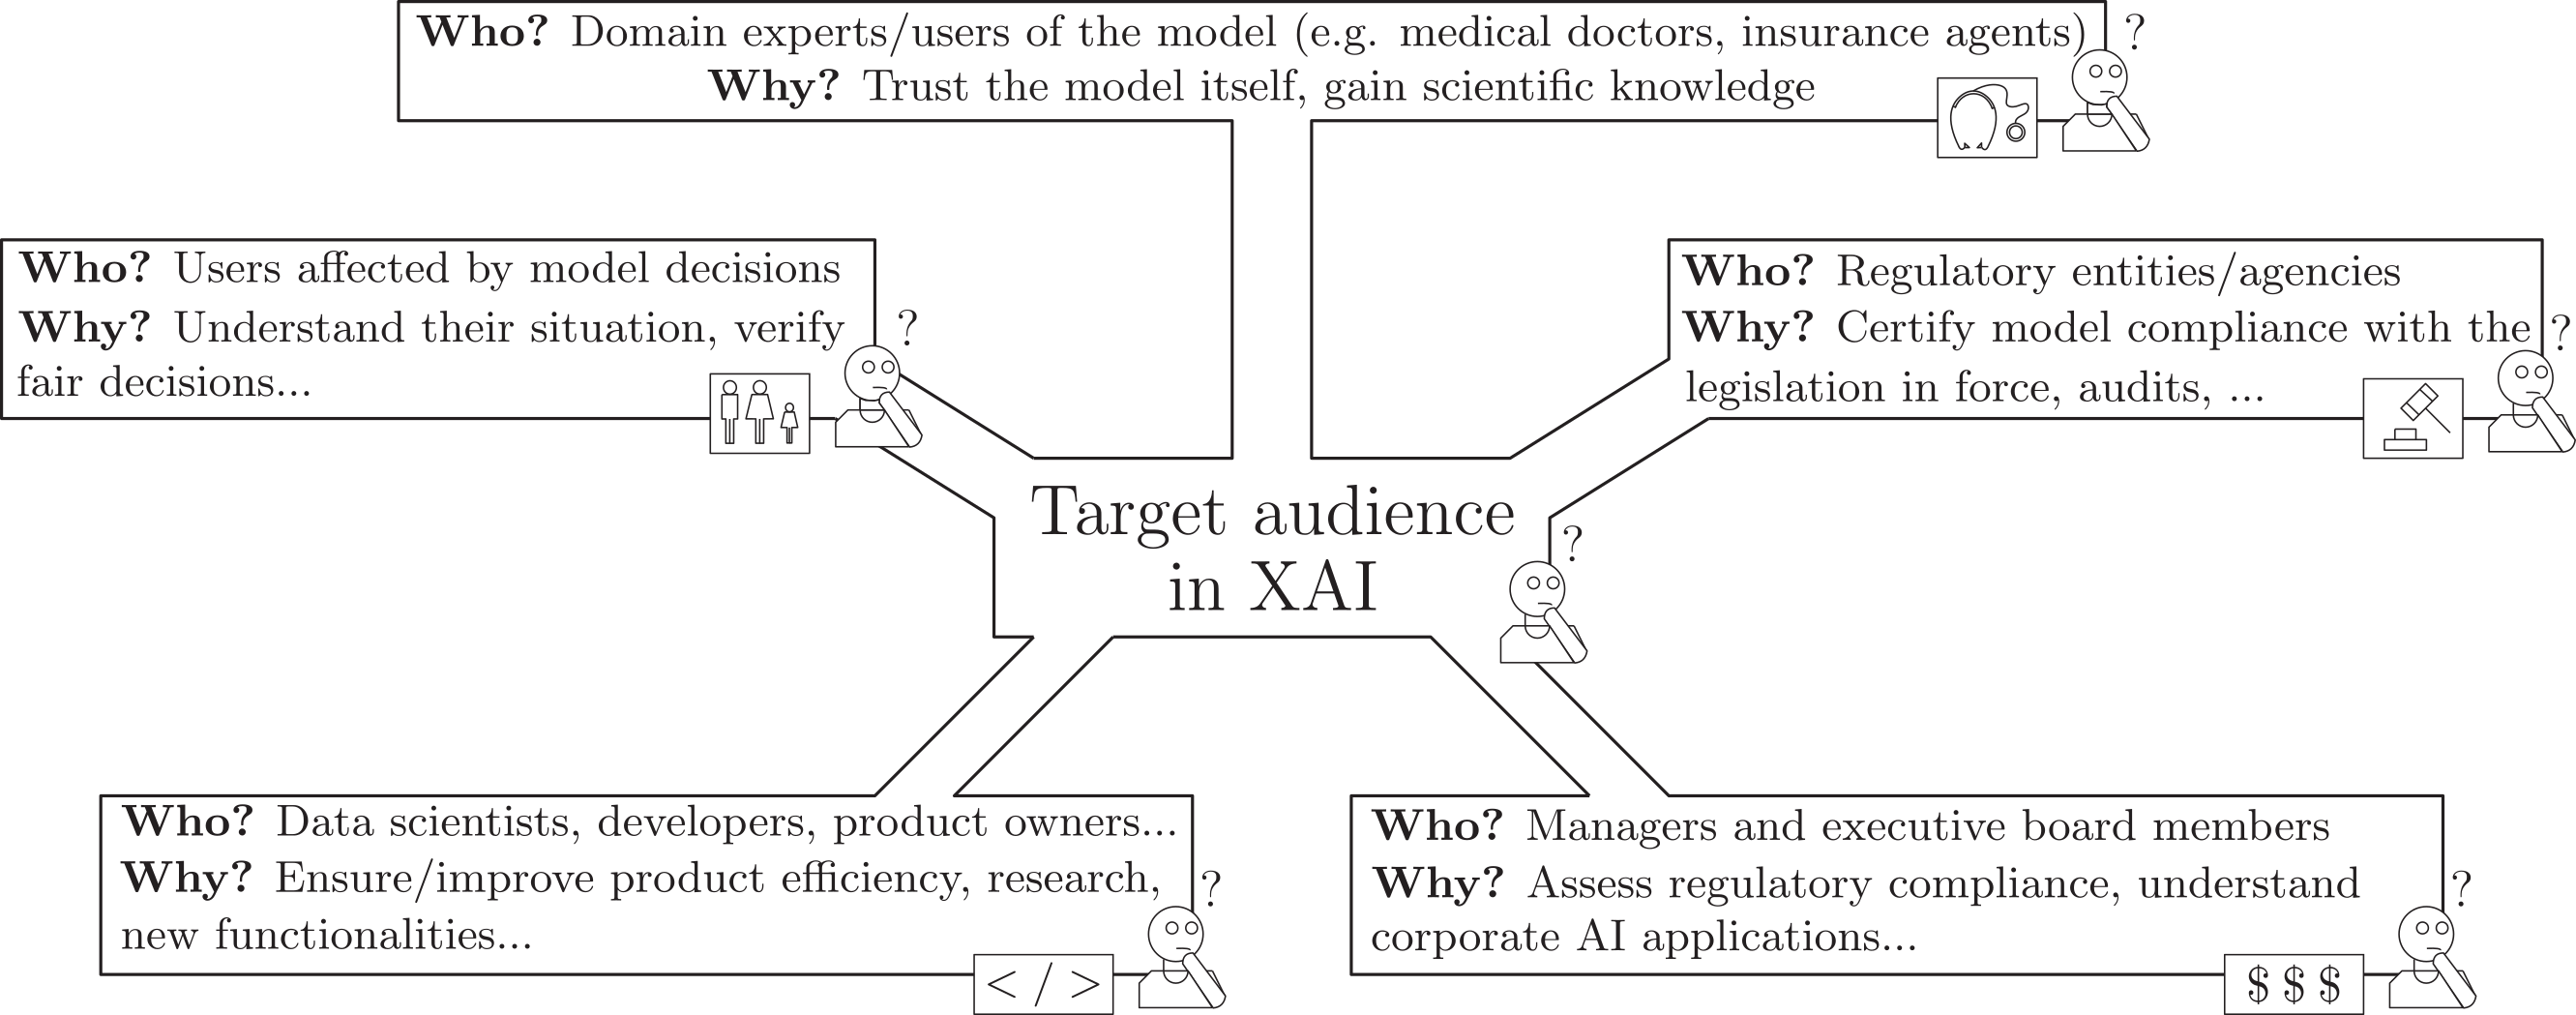
\includegraphics[scale = 0.65]{esquema_xai.png}
		\caption{Diagrama de las ventajas de la Inteligencia Artificial Explicable desde varios puntos de vista. Imagen de \cite{XAI}}
		\label{fig:esquema_xai}
	\end{figure}

\end{frame}

\section{Propuesta e implementación}
\begin{frame}{Conjunto de datos}

	\begin{columns}[T]
		\begin{column}{.5\textwidth}
			\vspace*{1cm}
			\begin{enumerate}
				\item 892 muestras: 439 de la lateralidad izquierda y 453 de la lateralidad derecha.
				\item Clasificadas manualmente por el Laboratorio de Antropología Física de la UGR.
				\item Altamente desbalanceado.
			\end{enumerate}
		\end{column}

		\begin{column}{.5\textwidth}
			\begin{figure}[H]
				\centering
				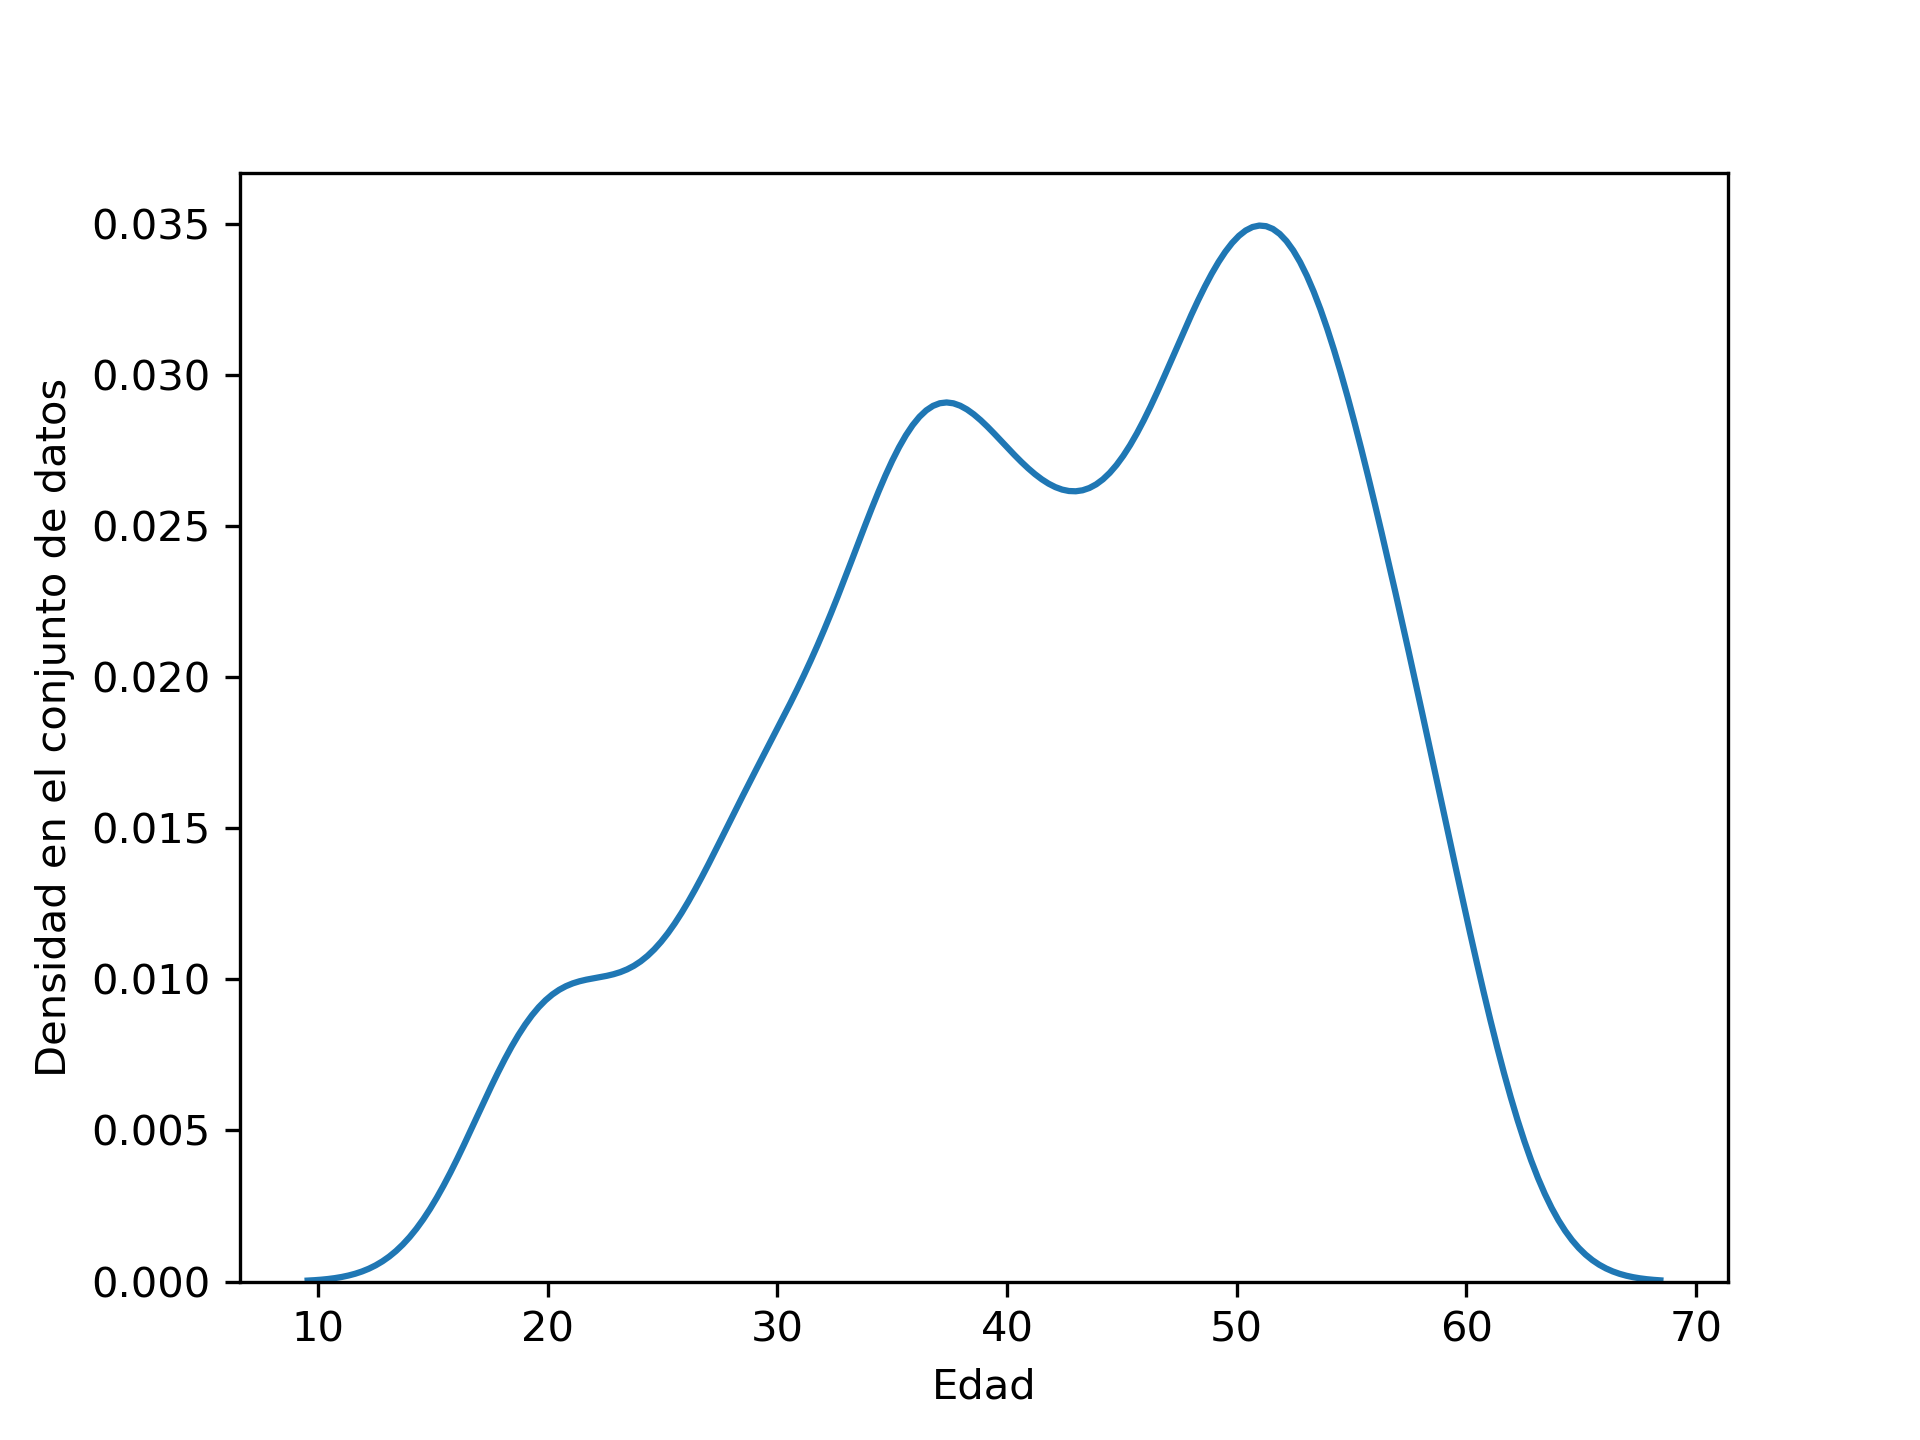
\includegraphics[width=1.15\textwidth]{completo_regresion.csv.png}
				\caption{Densidad de cada valor el conjunto de datos completo.}
				\label{fig:conjunto_regresion}
			\end{figure}
		\end{column}

	\end{columns}

\end{frame}

\begin{frame}{Enfoque utilizado}

	\begin{itemize}
		\item Enfoque de Gilbert y McKern, pero sin suma final de valores y utilizando las características propuestas por Todd.
		\item Regresión simbólica.
		\item Programación Genética y GA-P para aprender expresiones.
		\item Selección de características por parte del modelo.
		\item Sobremuestreo de datos utilizando SMOGN.
	\end{itemize}

\end{frame}

\begin{frame}{Algoritmos: Sobremuestreo de datos}
	SMOGN:

	\begin{columns}[T]
		\begin{column}{.5\textwidth}
			\begin{itemize}
				\item Mejora de SMOTER.
				\item SMOTER: Adaptación de SMOTE para regresión.
				\item Generación datos sintéticos utilizando un k-nn.
				\item Introducción de ruido gaussiano.
				\item Submuestreo aleatorio.
				\item Tiene en cuenta si es seguro y fiable generar un nuevo dato sintético.
			\end{itemize}
		\end{column}

		\begin{column}{.5\textwidth}
			\begin{figure}[H]
			    \centering
				 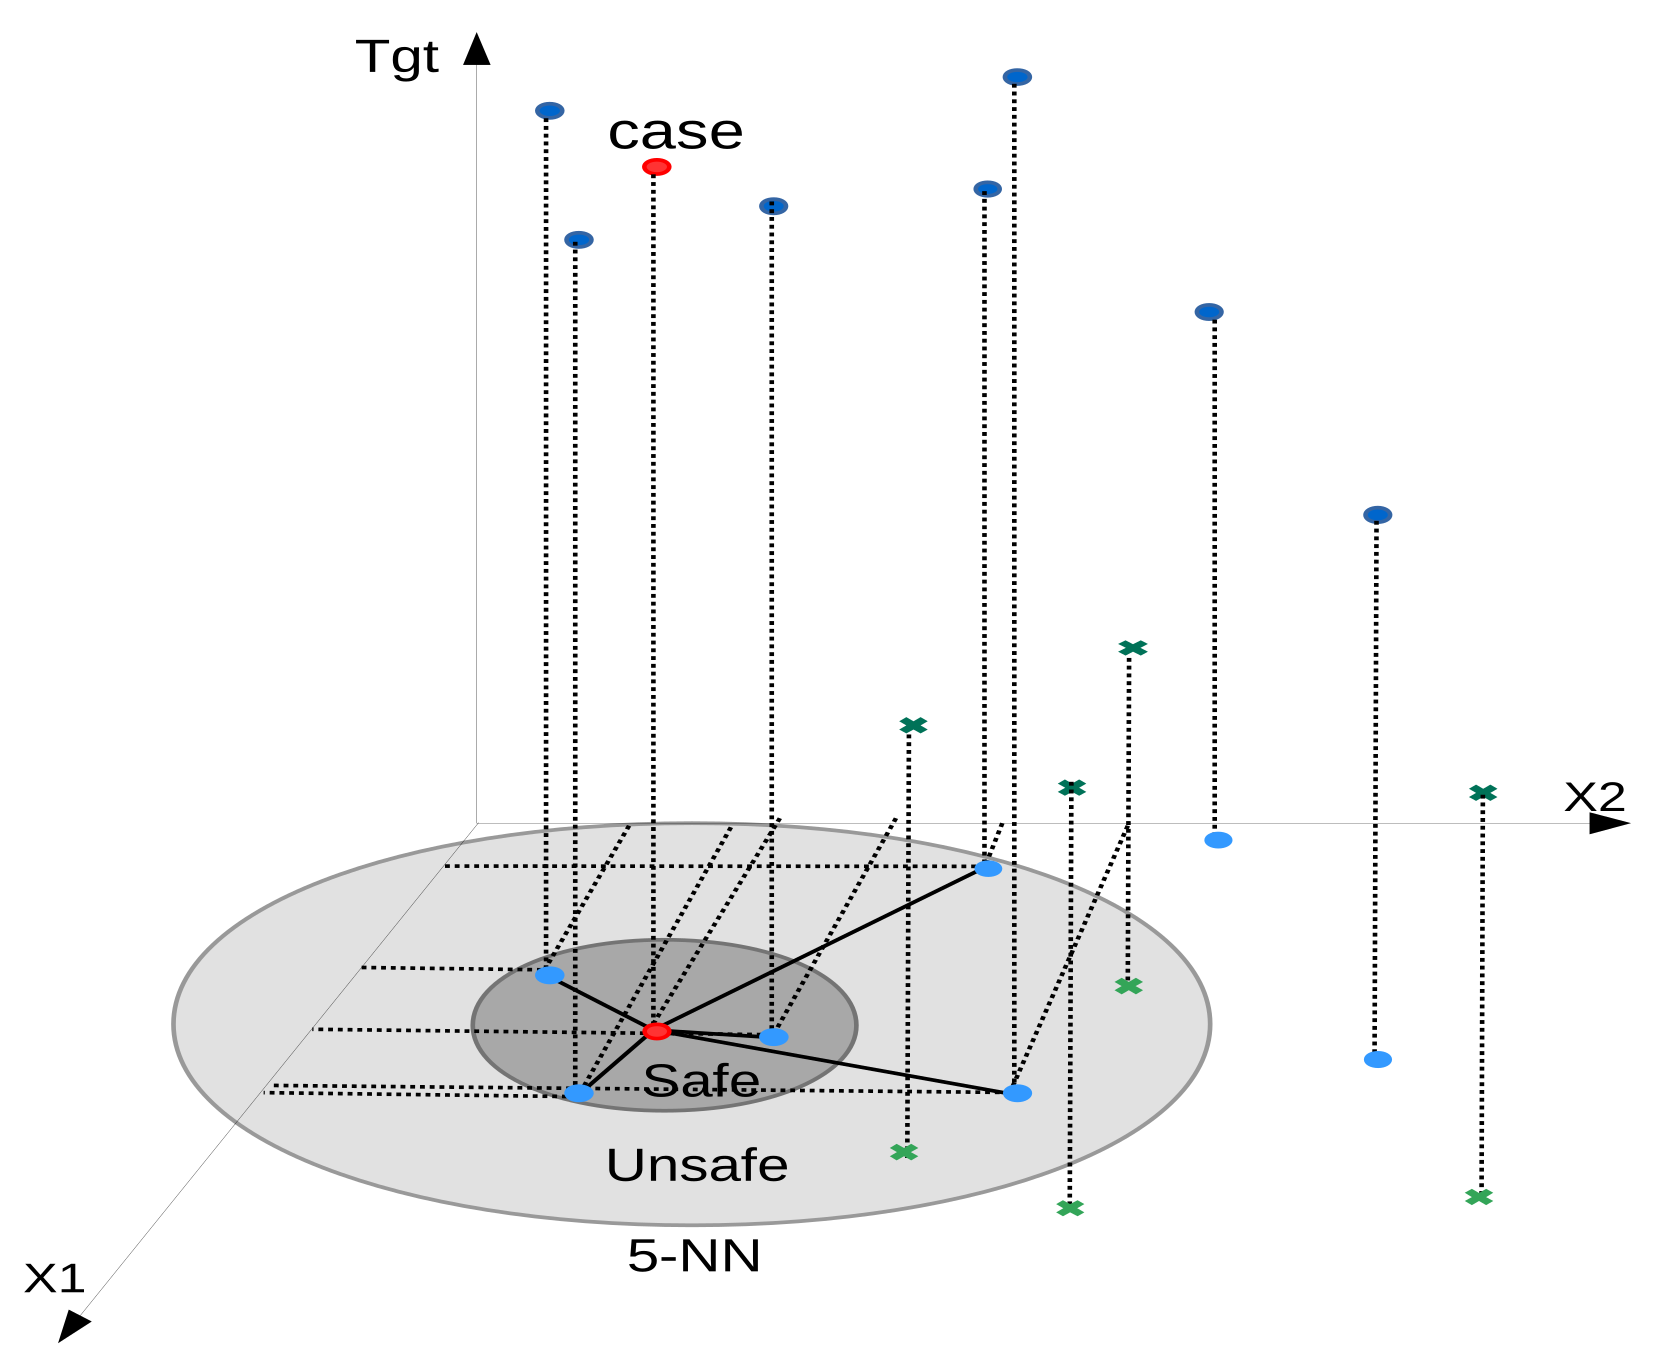
\includegraphics[width=\textwidth]{SMOGN-5NN.png}
			    \caption{Ejemplo de un dato sintético generado por SMOGN utilizando los cinco vecinos más cercanos. Imagen obtenida de \cite{SMOGN}}
				 \label{fig:SMOGN-5NN}
			\end{figure}
		\end{column}

	\end{columns}

\end{frame}

\begin{frame}{Algoritmos: Resultados tras sobremuestreo de datos}
		\begin{figure}[H]
			\centering
			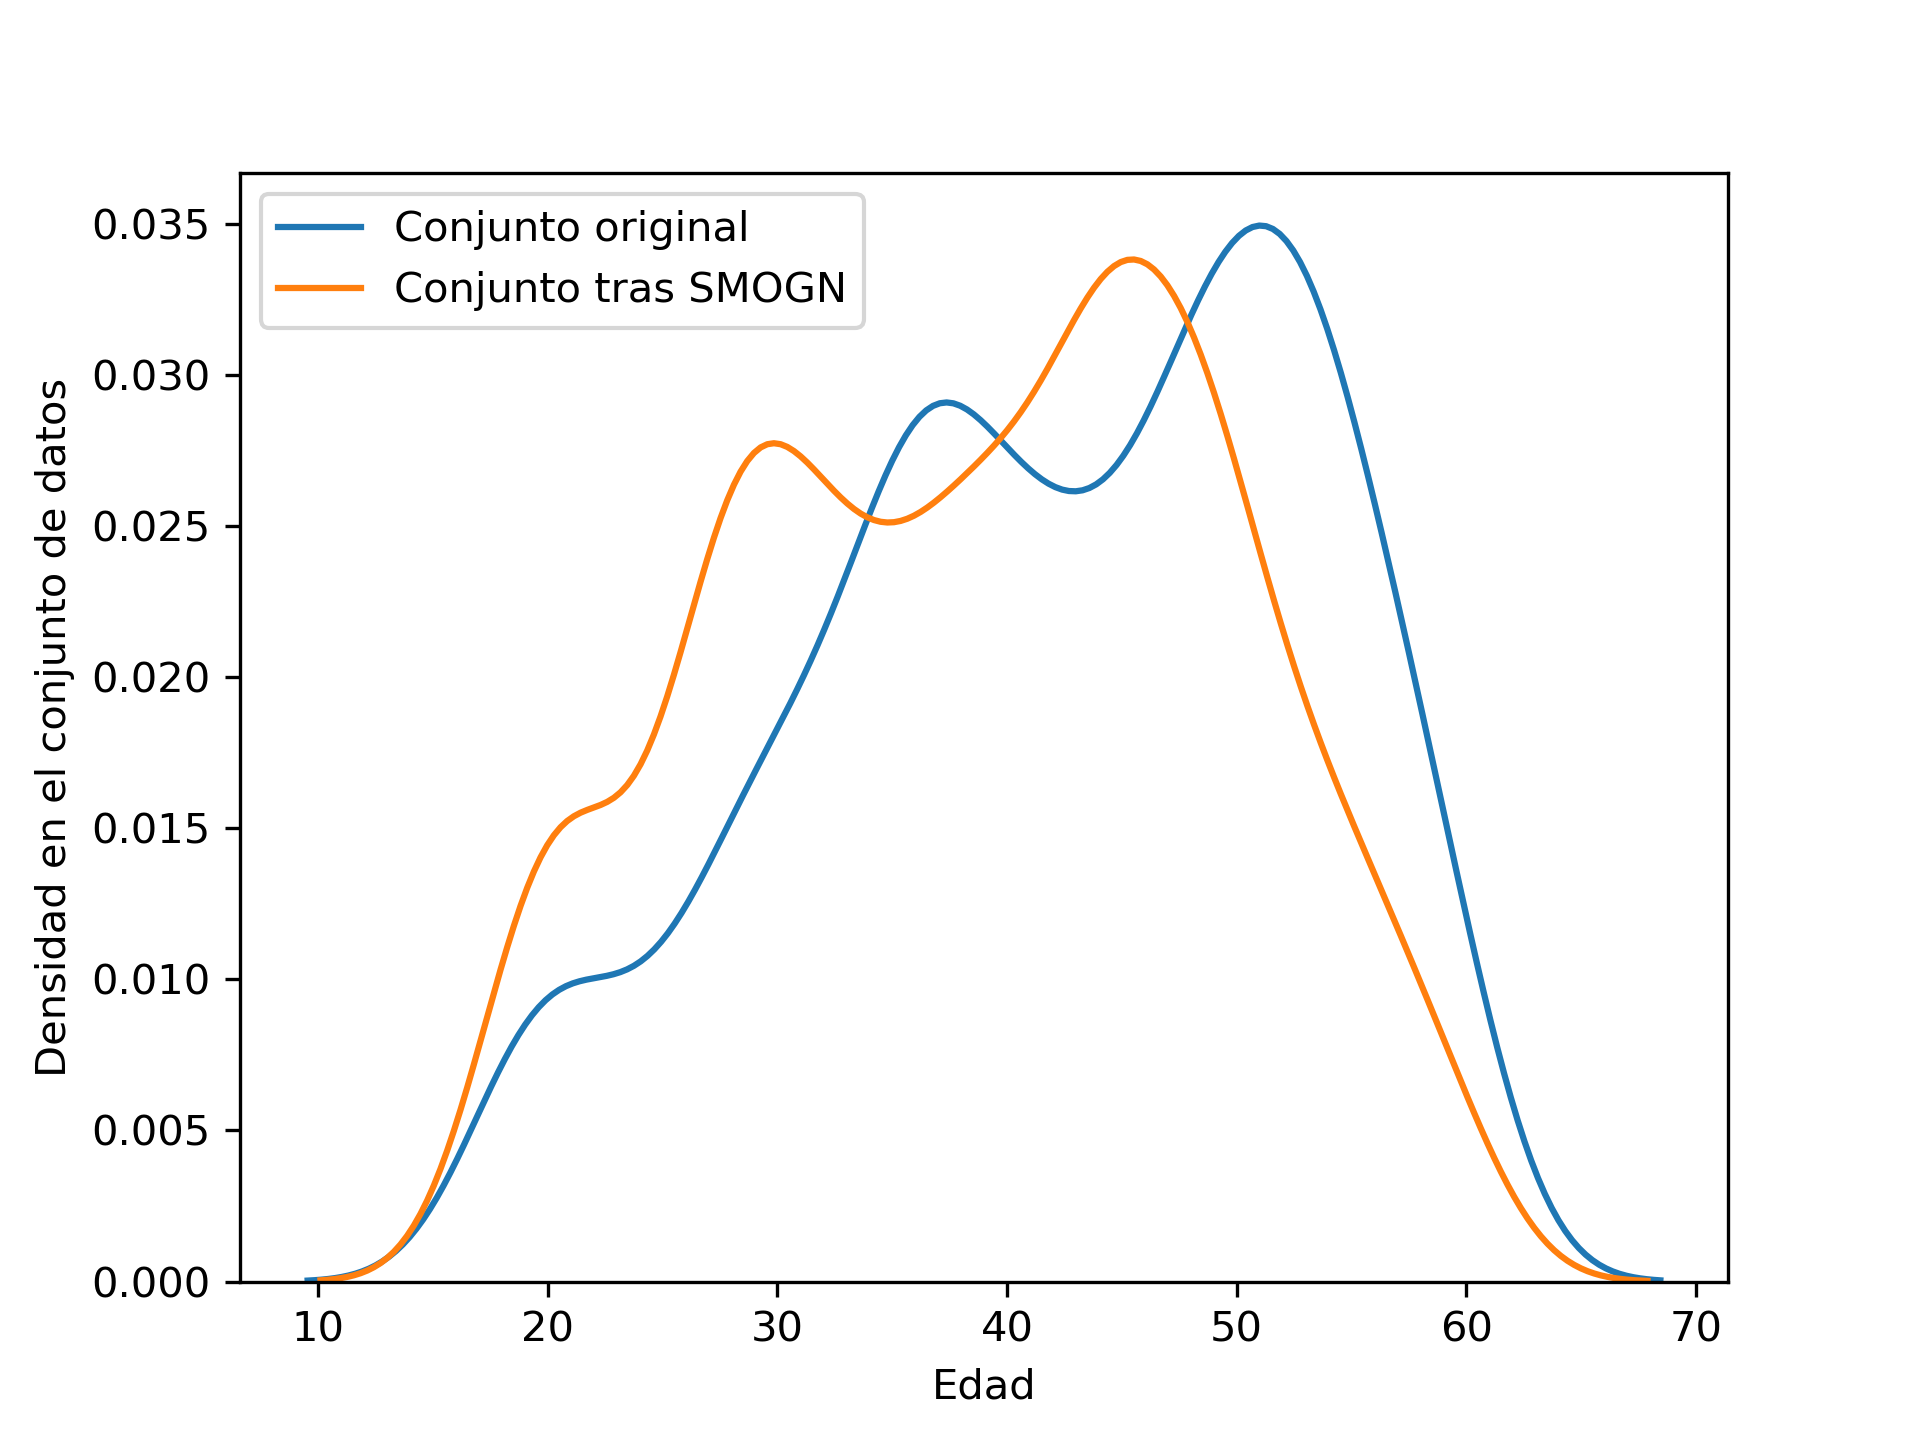
\includegraphics[width=0.8\textwidth]{tras_sobremuestreo.png}
			\caption{Resultados tras aplicar SMOGN sobre el conjunto completo.}
			\label{fig:tras_sobremuestreo}
		\end{figure}

\end{frame}

\begin{frame}{Algoritmos: Programación Genética}

	\begin{columns}[T]

		\begin{column}{.4\textwidth}
			\begin{itemize}
				\item Propuesto por John Koza en 1990 \cite{kozaGP}.
				\item Algoritmo evolutivo.
				\item Uso de árboles en lugar de cromosomas.
				\item Distintos tipos de problemas.
				\item Resultado: Árbol que mejor se ajusta a los datos.
				\item En nuestro caso, los árboles representan expresiones matemáticas.
			\end{itemize}
		\end{column}


		\begin{column}{.6\textwidth}
			\begin{figure}[H]
			    \centering
				 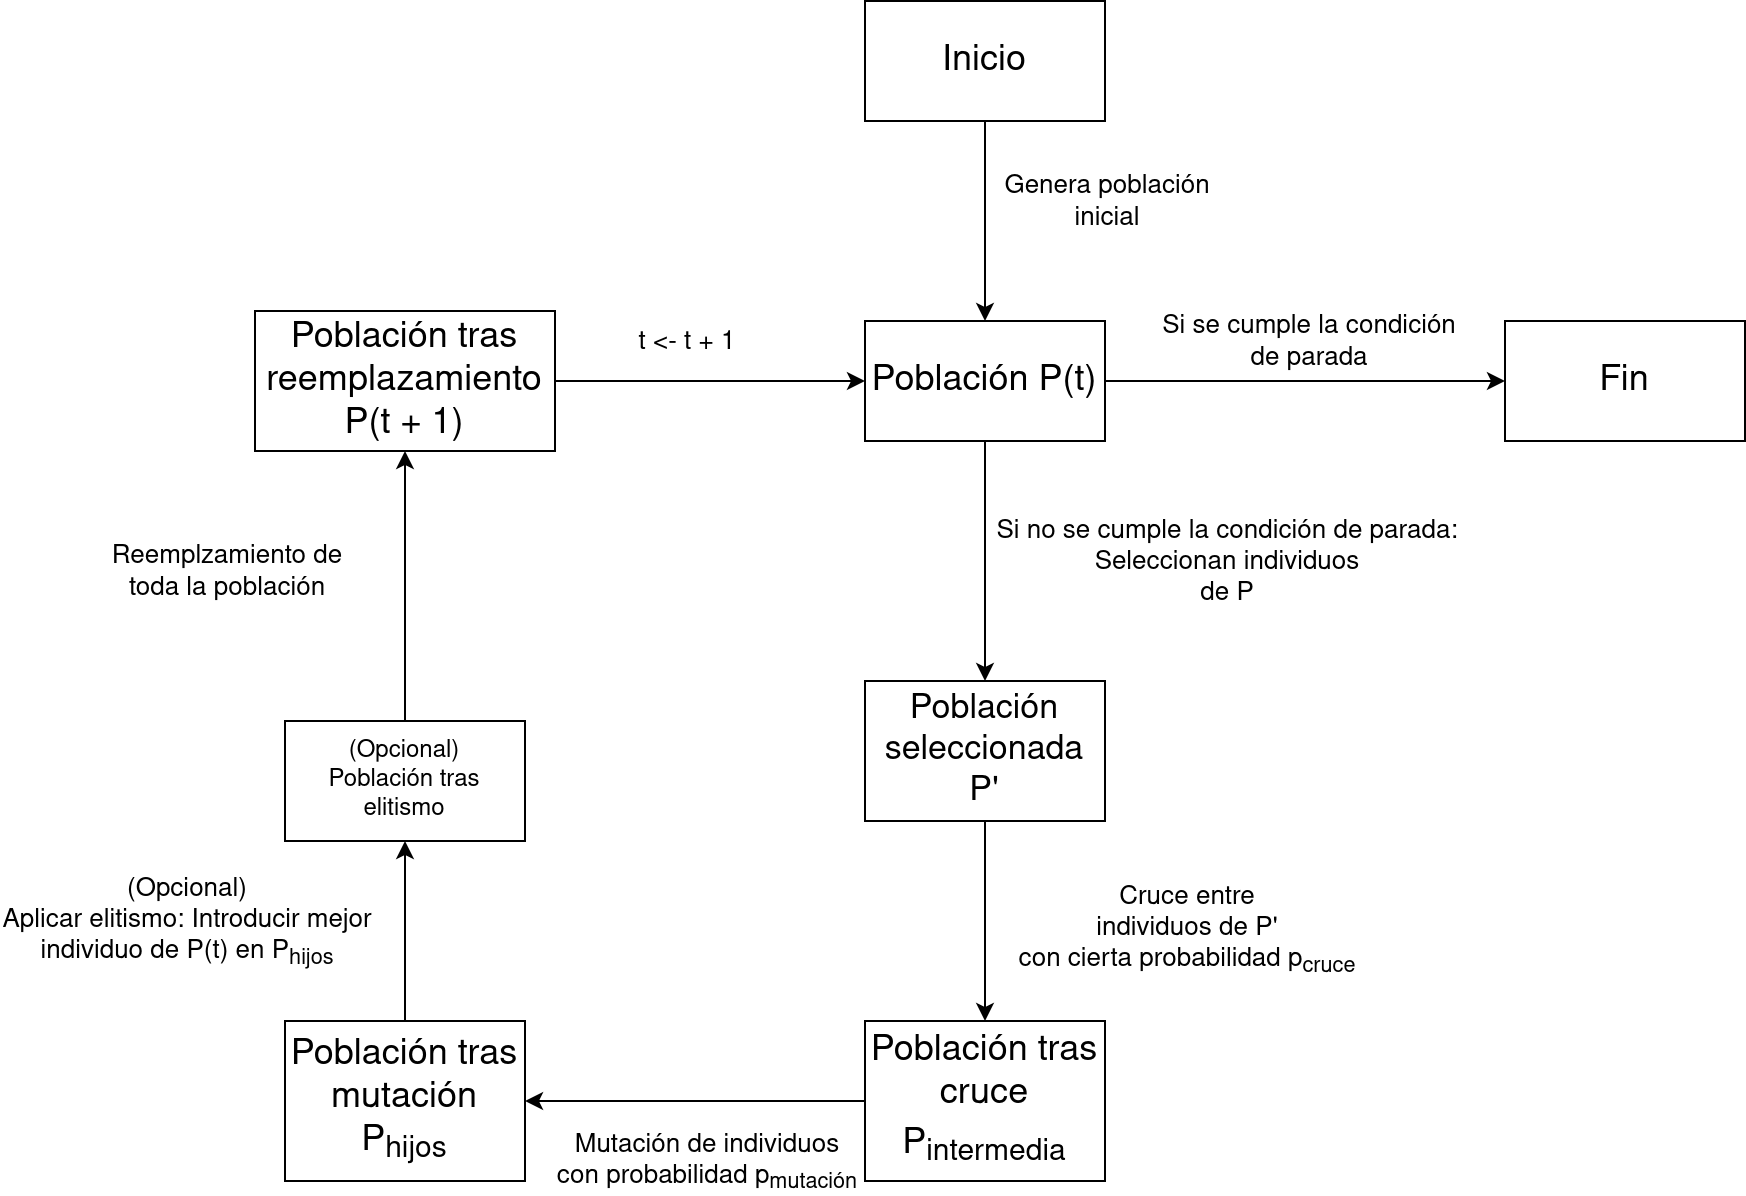
\includegraphics[width=\textwidth]{generacional.png}
			    \caption{Esquema de un algoritmo evolutivo con un modelo generacional.}
				 \label{fig:modelo_generacioal}
			\end{figure}
		\end{column}

	\end{columns}

\end{frame}

\begin{frame}{Algoritmos: GA-P}

	\begin{columns}[T]

		\begin{column}{.4\textwidth}
			\begin{itemize}
				\item Mejora de PG para regresión simbólica \cite{primerGAP}.
				\item Programación Genética para aprender expresiones y Algoritmo Genético para aprender constantes.
				\item Uso de nichos cuando las expresiones convergen.
			\end{itemize}
		\end{column}


		\begin{column}{.6\textwidth}
			\begin{figure}[H]
				\centering
				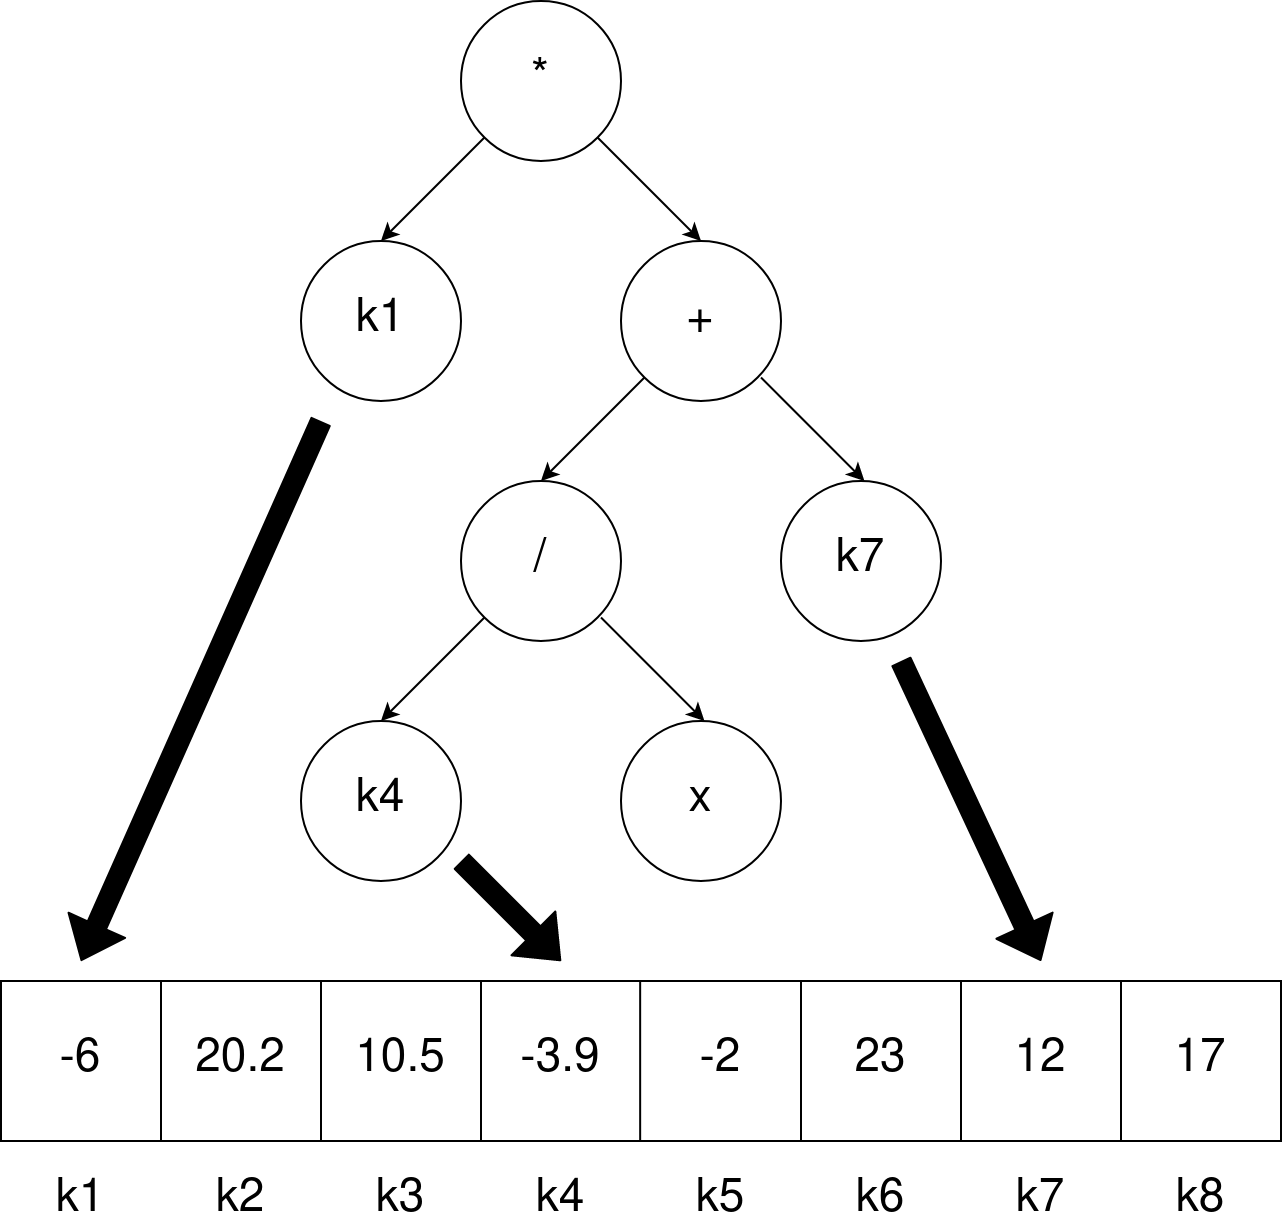
\includegraphics[width=0.6\textwidth]{expresion_gap.png}
				\caption{Ejemplo de una expresión de GA-P con un cromosoma asociado.}
				\label{fig:expresion_gap}
			\end{figure}
		\end{column}

	\end{columns}


\end{frame}

\begin{frame}{Algoritmos: Validación de los resultados}
	Uso de 5x2-\textit{cross validation}:

	\begin{itemize}
		\item 5 particiones distintas de los datos al $50\%$.
		\item Utilizamos la primera mitad para entrenar y la segunda para validar. Realizamos una segunda iteración intercambiando las dos mitades.
		\item Se obtienen 10 valores, 2 por cada partición.
		\item Resultado final: Media de dichos diez valores.
	\end{itemize}

\end{frame}

\begin{frame}{Tecnologías utilizadas}

	% Please add the following required packages to your document preamble:
	% \usepackage{graphicx}
	\begin{table}[H]
	\centering
	\resizebox{\textwidth}{!}{%
	\begin{tabular}{cc}
	
\includegraphics[width=0.13\textwidth]{logos/cpp.png} & 
\includegraphics[width=0.5\textwidth]{logos/python.png} \\
	
\includegraphics[width=0.3\textwidth]{logos/openmp.png} & 
\includegraphics[width=0.4\textwidth]{logos/googletest.png} \\
	\includegraphics[width=0.3\textwidth]{logos/doxygen.png} & 
\includegraphics[width=0.3\textwidth]{logos/git.png} \\
	
\includegraphics[width=0.4\textwidth]{logos/github.png} & 
\includegraphics[width=0.18\textwidth]{logos/github_pages.png}
	\end{tabular}%
	}
	\end{table}

\end{frame}

\section{Experimentos y análisis de resultados}

\begin{frame}{Experimentos}

	\begin{itemize}
		\item Seis conjuntos de datos.
		\item Tres longitudes máximas de árbol.
		\item Cinco semillas aleatorias distintas.
		\item Dos algoritmos: Programación Genética y GA-P.
		\item Ciento ochenta ejecuciones en total.
		\item Cada ejecución con un millón de evaluaciones y una población de mil individuos.
	\end{itemize}

\end{frame}


\begin{frame}{Comparación entre PG y GA-P}

	\begin{figure}[H]
	    \centering
		  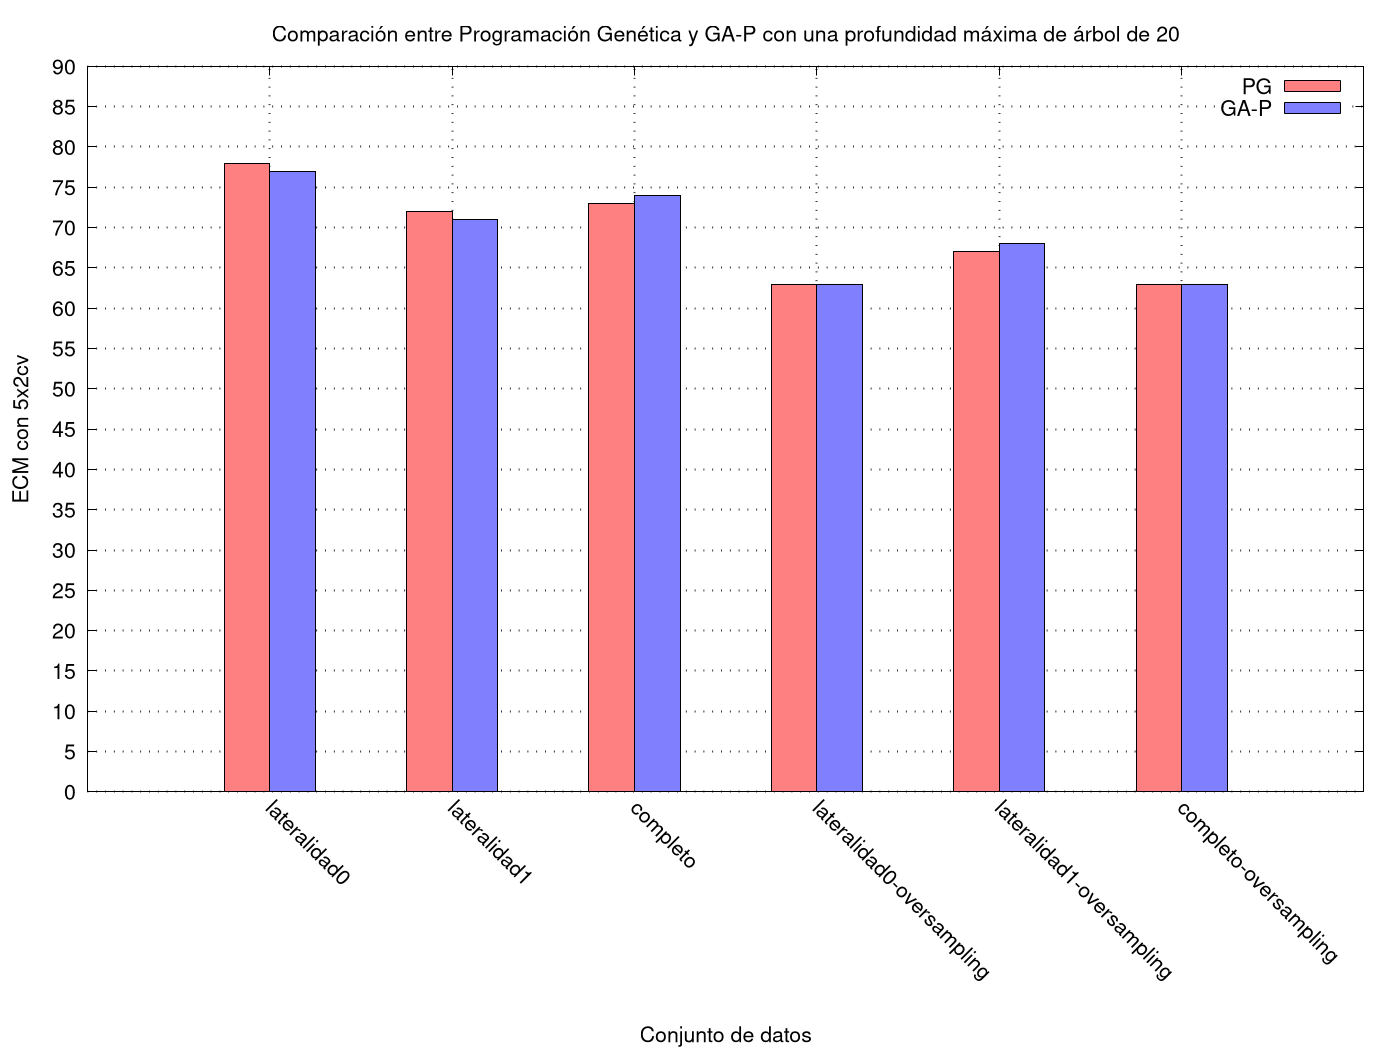
\includegraphics[width=0.7\textwidth]{comparacion_pg_gap_20.png}
		  \caption{Comparación entre PG y GA-P con longitud máxima de 20 nodos.}\label{fig:cmp_pg_gap_20}

	\end{figure}


\end{frame}


\begin{frame}{Importancia del sobremuestreo}

	\begin{figure}[H]
	    \centering
		  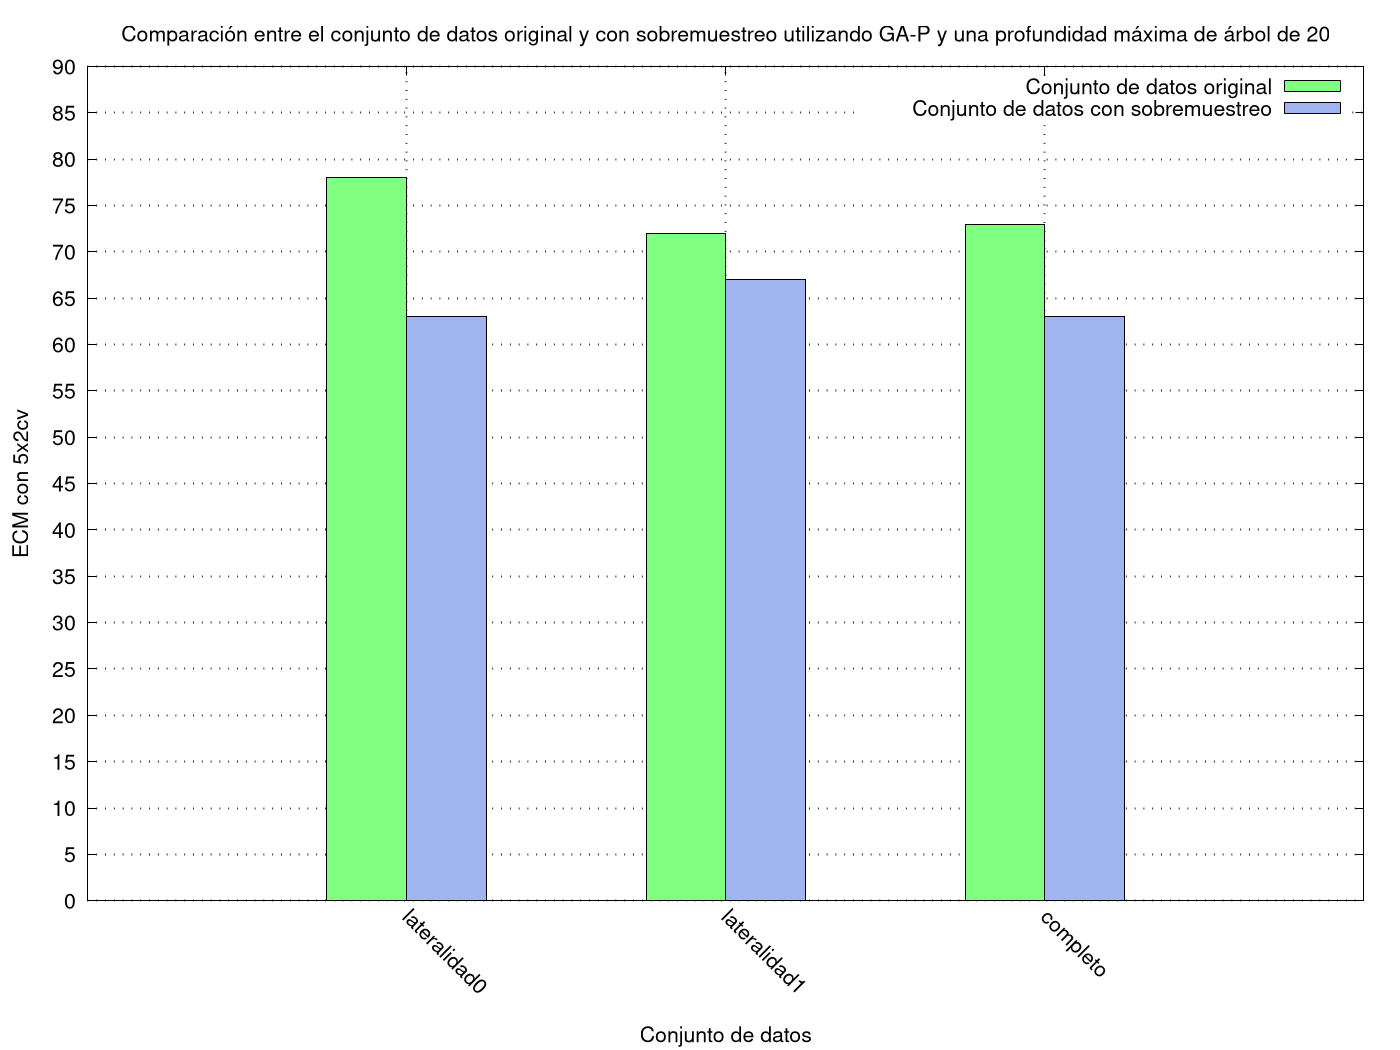
\includegraphics[width=0.7\textwidth]{comparacion_over_gap_20.png}
		  \caption{Comparación entre el conjunto de datos original y con sobremuestreo con GA-P y longitud máxima de 20 nodos.}\label{fig:cmp_gap_over_20}

	\end{figure}


\end{frame}

\begin{frame}{Mejores expresiones obtenidas}

	Mejor expresión obtenida por PG:
	\begin{equation} \label{eq:PG_completo}
	10.856 x_{4} + 5.428 x_{8} + 8.374 - \frac{3.803}{x_{1}^{3}}
	\end{equation}

	Mejor expresión obtenida por GA-P:
	\begin{equation} \label{eq:GAP_completo}
	2.330 x_{1} + 8.270 x_{8} + \left(x_{0} - x_{8}\right) \left(x_{8} - 2.330\right) + 16.945
	\end{equation}

	Mejor expresión obtenida por PG con sobremuestreo:
	\begin{equation} \label{eq:PG_completo_over}
	3.244 x_{1} - 3.244 x_{3} + x_{4}^{2} + 2.590 x_{4} x_{8} + 22.543
	\end{equation}

	Mejor expresión obtenida por GA-P con sobremuestreo:
	\begin{equation} \label{eq:GAP_completo_over}
	3.030 x_{1} + 5.632 x_{4} + 5.204 x_{8} + 12.212
	\end{equation}

\end{frame}


\begin{frame}{Uso de características}
	\begin{table}[H]
	\centering
	\resizebox{\textwidth}{!}{%
	\begin{tabular}{|c|c|c|c|c|c|c|c|c|c|c|}
	\hline
	\multicolumn{11}{|c|}{\textbf{Uso de variables}}                                                                                                                                                                                              \\ \hline
	                              & $\boldsymbol{x_0}$   & $\boldsymbol{x_1}$   & $\boldsymbol{x_2}$  & $\boldsymbol{x_3}$  & $\boldsymbol{x_4}$   & $\boldsymbol{x_5}$  & $\boldsymbol{x_6}$  & $\boldsymbol{x_7}$  & $\boldsymbol{x_8}$   & \textbf{\begin{tabular}[c]{@{}c@{}}Número total \\ de características\end{tabular}} \\ \hline
	\textbf{PG}                   & 46               & 94               & 14              & 8               & 64               & 12              & 42              & 57              & 105              & \textbf{442}                            \\ \hline
	\textbf{GA-P}                 & 48               & 93               & 20              & 10              & 68               & 14              & 60              & 42              & 85               & \textbf{440}                            \\ \hline
	\textbf{PG sobremuestreo}     & 54               & 94               & 13              & 17              & 67               & 18              & 29              & 22              & 97               & \textbf{411}                            \\ \hline
	\textbf{GA-P sobremuestreo}   & 44               & 80               & 25              & 21              & 67               & 35              & 27              & 29              & 86               & \textbf{414}                            \\ \hline
	\textbf{Total}                & \textbf{192}     & \textbf{361}     & \textbf{72}     & \textbf{56}     & \textbf{266}     & \textbf{79}     & \textbf{158}    & \textbf{150}    & \textbf{373}     & \textbf{1707}                           \\ \hline
	\textbf{\% respecto al total} & \textbf{11,25\%} & \textbf{21,15\%} & \textbf{4,22\%} & \textbf{3,28\%} & \textbf{15,58\%} & \textbf{4,63\%} & \textbf{9,26\%} & \textbf{8,79\%} & \textbf{21,85\%} & \textbf{}                               \\ \hline
	\end{tabular}%
	}
	\caption{Uso de las características en todas las fórmulas obtenidas dividido por algoritmo y sobremuestreo.}\label{table:uso_caracteristicas}
	\end{table}

\end{frame}



\begin{frame}{Comparación con el estado del arte}

	\begin{table}[H]
	\centering
	\resizebox{\textwidth}{!}{%
	\begin{tabular}{|c|c|c|c|}
	\hline
	\multicolumn{4}{|c|}{\textbf{Mejores resultados obtenidos en el estado del arte}}                                                                                        \\ \hline
	                                                                                                            & \textbf{Número de muestras} & \textbf{RECM} & \textbf{MAE} \\ \hline
	\textbf{Slice \& Algee-Hewitt \cite{modelandoHuesos3D}}                                    & 41                          & 17.15         & -            \\ \hline
	\textbf{Stoyanova,  Algee-Hewitt \& Slice \cite{mejoraModelandoHuesos3D}}                  & 57                          & 19            & -             \\ \hline
	\textbf{Stoyanova,  Algee-Hewitt, Kim \& Slice \cite{segundaMejoraModelandoHuesos3D}}      & 93                          & 13.7 - 16.5   & -             \\ \hline
	\textbf{Kotěrová, Navega, Štepanovský, Buk, Brůžek \& Cunha \cite{estimacionHuesosCadera}} & 941                         & 12.1          & 9.7          \\ \hline
	\end{tabular}%
	}
	\caption{Resultados obtenidos en los trabajos discutidos en el estado del arte.}\label{table:resultados_estado_arte}
	\end{table}

	\begin{table}[H]
	\centering
	\resizebox{0.5\textwidth}{!}{%
	\begin{tabular}{|c|c|c|}
	\hline
	\multicolumn{3}{|c|}{\textbf{Resultados de las expresiones escogidas}}   \\ \hline
	\textbf{}                       & \textbf{RECM}    & \textbf{MAE}        \\ \hline
	\textbf{PG (\ref{eq:PG_completo})}                     & 8,39821          & 6,92052             \\ \hline
	\textbf{GA-P (\ref{eq:GAP_completo})}                   & 8,4945           & 6,96785             \\ \hline
	\textbf{PG con sobremuestreo (\ref{eq:PG_completo_over})}   & 7,8669           & 6,41288             \\ \hline
	\textbf{GA-P con sobremuestreo (\ref{eq:GAP_completo_over})} & 7,87184          & 6,42334             \\ \hline
	\end{tabular}%
	}
	\caption{Resultados de las expresiones \ref{eq:PG_completo}, \ref{eq:GAP_completo}, \ref{eq:PG_completo_over} y \ref{eq:GAP_completo_over}.}\label{table:resultados_escogidas}
	\end{table}

\end{frame}



\section{Conclusiones}
\begin{frame}{Conclusiones}

	\begin{itemize}
		\item Propuesta prometedora para resolver un problema de gran interés y complejidad.
		\item Interés de uso de técnicas fácilmente interpretables, para a ayudar a los expertos.
		\item Estudio de distintas técnicas de preprocesado de datos.
		\item Revisión y propuesta de algoritmos evolutivos.
		\item Código documentado, escalable y reutilizable para otros trabajos.
		\item Estudio de resultados y comparación con el estado del arte, así como propuestas de trabajos futuros.
	\end{itemize}

\end{frame}

\section{Bibliografía}
\begin{frame}[allowframebreaks]{Bibliografía}

\begin{thebibliography}{9}

	\bibitem{todd}

	\href{https://onlinelibrary.wiley.com/doi/abs/10.1002/ajpa.1330030301}{\scriptsize T. W. Todd, “Age changes in the pubic bone,” American Journal of Physical Anthropology, vol. 3, no. 3, pp. 285–328, 1920.}

	\bibitem{propuestaGilbert}

	\href{https://onlinelibrary.wiley.com/doi/abs/10.1002/ajpa.1330380109}{\scriptsize Gilbert, B. M., \& McKern, T. W. (1973). A method for aging the female os pubis. American Journal of Physical Anthropology, 38(1), 31-38.}

	\bibitem{XAI}

	\href{https://www.sciencedirect.com/science/article/pii/S1566253519308103}{\scriptsize Arrieta, A. B., Díaz-Rodríguez, N., Del Ser, J., Bennetot, A., Tabik, S., Barbado, A., ... \& Herrera, F. (2020). Explainable Artificial Intelligence (XAI): Concepts, taxonomies, opportunities and challenges toward responsible AI. Information Fusion, 58, 82-115.}

	\bibitem{SMOGN}

	\href{http://proceedings.mlr.press/v74/branco17a/branco17a.pdf}{\scriptsize Branco, P., Torgo, L., \& Ribeiro, R. P. (2017, October). SMOGN: a pre-processing approach for imbalanced regression. In First international workshop on learning with imbalanced domains: Theory and applications (pp. 36-50). PMLR.}

	\bibitem{kozaGP}

	\href{https://mitpress.mit.edu/books/genetic-programming}{\scriptsize Koza, J. R., \& Koza, J. R. (1992). Genetic programming: on the programming of computers by means of natural selection (Vol. 1). MIT press.}

	\bibitem{primerGAP}

	\href{https://ieeexplore.ieee.org/stamp/stamp.jsp?tp=&arnumber=393137}{\scriptsize Howard, L. M., \& D'Angelo, D. J. (1995). The GA-P: A genetic algorithm and genetic programming hybrid. IEEE expert, 10(3), 11-15.}



	\bibitem{modelandoHuesos3D}

	\href{https://onlinelibrary.wiley.com/doi/full/10.1111/1556-4029.12778}{\scriptsize Slice, D. E., \& Algee‐Hewitt, B. F. (2015). Modeling bone surface morphology: a fully quantitative method for age‐at‐death estimation using the pubic symphysis. Journal of forensic sciences, 60(4), 835-843.}

	\bibitem{mejoraModelandoHuesos3D}

	\href{https://onlinelibrary.wiley.com/doi/full/10.1002/ajpa.22797}{\scriptsize Stoyanova, D., Algee‐Hewitt, B. F., \& Slice, D. E. (2015). An enhanced computational method for age‐at‐death estimation based on the pubic symphysis using 3 D laser scans and thin plate splines. American journal of physical anthropology, 158(3), 431-440.}


	\bibitem{segundaMejoraModelandoHuesos3D}

	\href{https://onlinelibrary.wiley.com/doi/full/10.1111/1556-4029.13439}{\scriptsize Stoyanova, D. K., Algee‐Hewitt, B. F., Kim, J., \& Slice, D. E. (2017). A computational framework for age‐at‐death estimation from the skeleton: surface and outline analysis of 3D laser scans of the adult pubic symphysis. Journal of forensic sciences, 62(6), 1434-1444.}

	\bibitem{estimacionHuesosCadera}

	\href{https://www.sciencedirect.com/science/article/pii/S0379073818301440}{\scriptsize Kotěrová, A., Navega, D., Štepanovský, M., Buk, Z., Brůžek, J., \& Cunha, E. (2018). Age estimation of adult human remains from hip bones using advanced methods. Forensic science international, 287, 163-175.}


\end{thebibliography}


\end{frame}


\section{Preguntas}


\end{document}
